\documentclass[a4paper,12pt]{scrreprt}
\usepackage[ngerman]{babel}
\usepackage{fontspec}
\usepackage[parfill]{parskip}
%\usepackage{eurosans}
\usepackage[top=3cm, left=3cm]{geometry}
\usepackage{setspace}
\usepackage{mdwlist}
\usepackage{graphicx}
\usepackage{eurosym}
\usepackage{pdfpages}
\usepackage{tikzsymbols}
\usepackage{footnote}
\usepackage{framed}
\usetikzlibrary{shapes}
\usepackage[autostyle=true]{csquotes}
\renewcommand*\familydefault{\sfdefault}



\definecolor{esebgcolor}{rgb}{1, 1, 1} % wip-ish color -- #0D5F98
\definecolor{esefgcolor}{rgb}{0,0,0}

\setcounter{secnumdepth}{-1}
\setcounter{tocdepth}{1}
\begin{document}

\title{\huge{\textbf{Vor dem Tutorium lesen und wichtige Punkte markieren!}}\\\ \\\ \\{Leitfaden für ESE-Tutoren 2020}}


\date{}

\author{}
\maketitle

\section*{\enquote{Anwesenheit} in der ESE}
Eure Anwesenheit ist zu folgenden Zeiten ausdrücklich erforderlich:
\begin{itemize*}
    \item Aufgabenbereiche, in denen ihr explizit als Helfer eingetragen seid
    \item Einschreibung am Dienstag
    \item Campusschnitzeljagd am Dienstag
    \item ESE-Spiel am Freitag
\end{itemize*}
Wichtig für die einzelnen Termine sind auch die vorherigen Tutorenbriefings im bbb. Diese sind unbedingt zu besuchen und werden bei Nichterscheinen mit dem Nichtmögen von Engeln geahndet.\\
\begin{itemize*}
    \item Montag        08:00 Uhr
    \item Dienstag      08:00 Uhr und 14:00 Uhr
    \item Freitag       13:00 Uhr
\end{itemize*}

Die Anwesenheit zu allen anderen Veranstaltungen ist wünschenswert!

\section*{Aufgaben eines ESE-Tutors}

\begin{itemize*}
    \item \textbf{Proud to be a Tutor:} Trage während der Woche zu allen ESE-Veranstaltungen (auch abends) das ESE-Shirt und dein Namensschild.
    \item \textbf{Sei hilfsbereit:} Siehst du einen einsamen Ersti, hilf ihm, Anschluss zu finden. Ein Ersti fragt dich etwas oder ein Ersti guckt sich verloren um? Setze alles daran zu helfen!
\end{itemize*}

\section*{Erreichbarkeit der ESE-Orga}

Solltet ihr Probleme oder Fragen haben, meldet euch bitte bei der ESE-Orga.

Während der ESE-Woche sollte immer ein Orga-Mitglied im Büro sitzen.
Außerdem erreicht ihr die ESE-Orga
\begin{itemize*}
    \item per Mail: ese-orga@ifsr.de
    \item telefonisch: 0351/463-38226
\end{itemize*}


\tableofcontents
\chapter{Hinweise für Tutoren}

\section{Über das Tutorium}
Ziel des Tutoriums ist die Vermittlung von Informationen rund um das Studium. Der Inhalt dieser Handreichung ist das Minimum, was ihr in den Tutorien vermitteln sollt. Ihr könnt die Stichpunkte gerne noch mit eigenen Einfällen ergänzen.\\
Beachtet dabei:
\begin{itemize*}
\item Die Informationen sollten möglichst \textbf{unparteiisch} und \textbf{nicht wertend} vermittelt werden.
Insbesondere sollte man vermeiden, den Erstis schon vorab Angst vor bestimmten Vorlesungen oder Dozenten zu machen oder sie zum Nichtbesuchen der Vorlesungen zu animieren. Das betrifft auch das ESE-Spiel.
\item Eine Tutoriengruppe besteht aus zwei Tutoren und ca. 15--25 Erstis.
\item Solltet ihr zu einem der Themen keine Ahnung haben, dann verweist auf den FSR\@.
\end{itemize*}

\section{Vor dem Tutorium zu erledigende Dinge}
\begin{itemize*}
    \item Überlegt euch, wie ihr die Informationen vortragen wollt.
    %\item Den Raum bitte vorher schon mal suchen, falls ihr nicht sicher wisst, wo er sich befindet.
    \item Sucht euch einen geeigneten Ort, von dem aus ihr zu zweit vor einer Webcam stehen könnt.
    \item Am ESE-Montag zum Briefing um 08:00 da sein!
\end{itemize*}


\chapter{In den Tutorien zu vermittelnde Informationen}

\section{Ablaufplan}

\begin{itemize*}
    \item Einführung
    \item Überblick ESE-Woche
    \item Kennenlernen
    \item Außerhalb vom Studium
\end{itemize*}

\section{Einführung}
\begin{itemize*}
    \item Wenn ihr Masterstudierende in eurer Gruppe habt, schickt sie in den entsprechenden bbb.
    \item Motiviert die Studierenden, den Videochat zu starten, damit es persönlicher wird. Es sollte niemand gezwungen werden, sein Gesicht zu zeigen, es ist aber für den ersten Kontakt zu Kommilitonen hilfreich.
    \item \textbf{Wichtig!} Hierbei geht es nicht um das Studium. Versucht deshalb Fragen zum Studiengang zu vermeiden.
    \item Schreibt eure Emailadressen in den chat, für Nachfragen.
    \item Erzählt etwas zu eurem Namenspatron. Informationen findet ihr im Anhang.
    \item \textbf{!!~Am Wichtigsten~!!} Der Check-In Bereich der Webseite gibt zu jeder Veranstaltung die notwendigen Anweiseungen. Dieser sollte mehrmals eindrücklich erwähnt werden.
\end{itemize*}

\pagebreak

\section{Überblick ESE-Woche}

\begin{framed}
Auf der ESE-Webseite (https://ese.ifsr.de) befindet sich der jeweils aktuelle Ablaufplan, Weblinks und Infos zum Studium. Kurzfristige Änderungen und Ankündigungen werden via Twitter (@ifsr) bekanntgegeben.
\end{framed}

\begin{itemize*}
%    \item Den Zeitplan gibts auch im iCal-Format (ICS Datei) zum Download.
%    Kann man sich direkt in den Kalender importieren.
    \item Da die Studierenden ihre Beutel noch nicht erhalten habt, weist bitte auf die online version von \enquote{The Manual} hin (auf der ESE webseite verlinkt).
    \item Geht die ESE-Woche durch und sagt kurz etwas zu den wichtigsten Programmpunkten.
    \item Bitte betont nochmal, dass die ESE sehr gut geeignet ist, um Kommilitonen kennenzulernen.
\end{itemize*}

% TODO Plan von unten Einfügen und Kommentare auf Seite daneben

\subsection{Der Rest von Montag}

\textbf{Vorstellung der Lehrenden}
\begin{itemize*}
    \item Passiert genau wie die Einführungsveranstaltung via Stream.
\end{itemize*}

\textbf{Speedfriending}
\begin{itemize*}
    \item beginnt 17:00, dauert die gesamte ESE an.
    \item \texttt{friends.ese.ifsr.de} bildet Jitsiräume mit zwei Teilnehmenden. Link dazu auf der Webseite.
    \item Die Maximaldauer eines Gespräches wird nicht enforced. Die Studierenden sollen selbst darauf achten, sich hin und wieder neu zuweisen zu lassen.
\end{itemize*}


\subsection{Dienstag}

\textbf{Einschreibung}
\begin{itemize*}
    \item Die Systeme zur Einschreibung in Veranstaltungen werden vorgestellt.
    \item \textbf{!!~WICHTIG~!!} Es gibt in diesem Jahr keine Stundenpläne.
    \item \texttt{distribute.ese.ifsr.de} bildet Jitsiräume mit je einem Engel und einem Ersti. Link dazu auf der Webseite.
    \item Durchschnittliche Einschreibezeit liegt bei 10 Minuten.
    \item Wartezeiten sollten eingeplant werden.
\end{itemize*}

\textbf{Vorträge zu Auslandsaufenthalt und Studentischer Selbstverwaltung}
\begin{itemize*}
    \item Passiert genau wie die Einführungsveranstaltung via Stream.
\end{itemize*}

\textbf{Campusschnitzeljagd}
\begin{itemize*}
    \item Realisiert durch \texttt{gather.town}. Link dazu auf der Webseite.
    \item \texttt{gather.town} ist ein custom 2d Spiel mit Positional audio.
    \item Nach Klick auf den Link gibt es eine Anleitung. Sollte alles selbsterklärend sein.
\end{itemize*}

\textbf{Clubwanderung}
\begin{itemize*}
    \item Beginn 19:00 Uhr am Club Countdown (Güntzstraße 22).
    \item In kleinen Gruppen wird mit Hygienekonzept die Dresdner Studierendenclubszene erkundet.
    \item Ein Engel ist dabei.
    \item \textbf{Anmeldung über Kurssystem.}
\end{itemize*}


\subsection{Mittwoch}

\textbf{Wanderung}
\begin{itemize*}
    \item Verschiedene kleine Gruppen (10 Menschen) mit unterschiedlichen Schwierigkeitsgraden.
    \item \textbf{Anmeldung über Kurssystem.} Dort gibts alle Infos.
    \item Verschiedene Gruppen haben verschiedene Abfahrten.
\end{itemize*}


\textbf{Spieleabend}
\begin{itemize*}
    \item Findet in Präsenz am Mittwoch und Donnerstag abend statt.
    \item Maximal 80 Teilnehmer.
    \item \textbf{Anmeldung über Kurssystem.}
    \item ascii stellt sich vor. Erster Cocktail frei.
    \item agdsn stellt sich vor. Erster Tschunk frei.
    \item 20:15 Filmvorführung \enquote{Im Toten Winkel} mit Einführung der Filmemacher für maximal 20 Personen.
\end{itemize*}


\subsection{Donnerstag}
\textbf{Vorträge zum Studium}
\begin{itemize*}
    \item Vorträge zu Studienangelegenheiten und Sprachkursen
    \item Passiert genau wie die Einführungsveranstaltung via Stream.
\end{itemize*}

\textbf{Nerd::101}
\begin{itemize*}
    \item Workshops zu themen, die Informatikstudierende ganz gut gebrauchen können
    \item Finden in bbb statt. Links zu den einzelnen Workshops auf der Webseite.
\end{itemize*}

\textbf{Spieleabend}
\begin{itemize*}
    \item siehe Spieleabend Mittwoch
\end{itemize*}

\pagebreak

\subsection{Freitag}
\textbf{Seminargruppentreffen}
\begin{itemize*}
    \item Wichtige Informationen rund um das Studium. Noch detaillierter als vorher.
    \item Allgemeiner Sinn der Seminargruppen: Unterstützung der Erstis, Gruppenbildung, Mentor als Ansprechpartner bei Problemen und Vermittlung aller relevanten Informationen zum Studiengang
    \item Bitte betonen: An allen Treffen teilnehmen!
    \item Finden in bbb statt. Links dazu auf der Webseite.
    \item Ersties müssen sich vorher in Seminargruppe über \texttt{kurse.ifsr.de} eingeschrieben haben.
    \item Seminargruppentreffen starten ALLE um 10:00 Uhr
\end{itemize*}

\textbf{ESE-Spiel}
\begin{itemize*}
    \item Simulation des gesamten Studiums in spielerischer Form.
    \item Findet auf dem Minetest server der ESE statt: \texttt{pet.ifsr.de}.
    \item Anleitung gibts auf der Webseite. Erklärt sich von selbst.
\end{itemize*}


\textbf{Neustadt Kneipentour}
\begin{itemize*}
    \item \textbf{Anmeldung über Kurssystem.}
    \item Bei Anmeldung nur Preferenzen auswählen. Gruppen werden vor Ort gebildet.
\end{itemize*}


\subsection{Samstag}

\textbf{Stadtführung}
\begin{itemize*}
    \item DIY Stadtführung. Bitte Gruppen suchen und bereitgestellte Routen ablaufen. Infos auf der Webseite.
\end{itemize*}

\section{Danach}
\subsection{Mensakarten}
\begin{itemize*}
    \item Können ab erster Semesterwoche beim FSR APB/E017 abgeholt werden.
    \item \EUR{5} Pfand benötigt.
    \item E-Meal Bescheinigung und Ausweis mitbringen
\end{itemize*}

\subsection{ESE-Beutel}
\begin{itemize*}
    \item Können ab erster Semesterwoche beim FSR \texttt{APB/E017} abgeholt werden.
    \item Enthalten tolle goodies. Wurde vorher im Stream unboxed.
    \item Enthält vor Allem \textbf{The Manual}.
\end{itemize*}


\section{Kennenlernen}
\begin{itemize*}
    \item Dieser Punkt ist der Hauptfokus neben der Informationsvermittlung, lasst euch dafür ausreichend Zeit.
    \item Versucht ein lockeres Gespräch aufzubauen!
    \item Spielt gemeinsam mit den Erstis ein paar Spiele zum Kennenlernen
    \item Im Folgenden haben wir für euch ein paar Ideen für Spiele aufgelistet, die ihr mit den Erstis so in der Reihenfolge machen KÖNNT, d.h.\ wenn Ihr kreativ seid, dann könnt Ihr euch selbst Spiele ausdenken
\end{itemize*}


\subsection{Kennlernspiele}

\subsubsection{Human Sort}
\begin{itemize*}
    \item Stellt euch mit den Erstis nach verschiedenen Sortierungskriterien in einer Reihe auf, z.B. sortiert nach
    \item \dots dem Abstand von eurem Geburtsort zu Dresden
    \item \dots dem Zeitpunkt wann ihr das erste Mal an einem Rechner genutzt habt
    \item \dots der geschätzten voraussichtlichen Studienzeit
\end{itemize*}

\subsubsection{Unionize!}
\begin{itemize*}
    \item Legt 3-4 Kategorien fest, wie z.B. Lieblingsessen, Welches Tier wärst du am liebsten, Hobbies
    \item Schreibt Stichpunkte zu den Kategorien auf einen Zettel
    \item Findet größtmögliche Gruppen von Erstis mit Gemeinsamkeiten
    \item Überlegt euch Gruppennamen
    \item Stellt die Gruppen vor
\end{itemize*}

\subsubsection{Gegenseitiges Vorstellen}
\begin{itemize*}
    \item Legt drei Vorstellungsfragen fest, wie z.B. Was ist deine Mission? Was machst du am Liebsten am Rechner? Wohin willst du?
    \item Findet euch paarweise zusammen
    \item Stellt euch gegenseitig vor und beantwortet die Fragen
    \item Alle beantworten die Fragen für die jeweils andere Person in der ganzen Gruppe
\end{itemize*}

\pagebreak

\section{Außerhalb des Studiums}

\subsection{Wohnen in Dresden}
\begin{itemize*}
    \item neuen Wohnsitz innerhalb von 14 Tagen melden
    \item Hauptwohnsitz nach Dresden verlegen $\rightarrow$ \EUR{150} \enquote{Begrüßungsgeld}\\
    $\rightarrow$ beantragen beim Studierendenwerk
    \item Zweitwohnungssteuer in Dresden seit 2006 fällig. Bewohner einer WG oder eines Wohnheims kann Widerspruch einlegen
    \item Fragt wer in welchen Stadtbezirken wohnt, damit die Erstis Nachbarn in ihrer Nähe kennenlernen
\end{itemize*}

\subsection{Essen}
\begin{itemize*}
    \item Emeal-Karte zum Zahlen in allen Mensen und Cafeterien der TU Dresden
    \item erhältlich in den Mensen oder im FSR-Büro.
    $\rightarrow$ Emeal-Bescheinigung (Imma-Bogen), \EUR{5} Kaution, Studierendenausweis, Ausweis mitbringen
    \item Aufladen am Automaten in den großen Mensen, an der Kasse (zum Teil nur mit Bargeld möglich), auf Wunsch per Autoload
    \item Karte mit Mensen zeigen
    \item Alternativen zu den Mensen in der Nähe
    \begin{itemize*}
        \item Firat, Dersim
        \item Konsum und Bäckerei Möbius am Münchner Platz
        \item dm, Netto und Bäckerei Schmidt am Nürnberger Platz
        \item Müsli, belegte Brötchen, Donuts und Snacks im ASCII
    \end{itemize*}
\end{itemize*}

\subsection{Engagment}

\subsubsection{ASCII}
\begin{itemize*}
    \item Das Studierendencafe in der Informatik Fakultät, gleich neben dem FSR Büro
    \item Wird von einem Verein betrieben, bei dem ihr unkompliziert Mitglied werden könnt und ist auf Unterstützung von Studierenden angewiesen
\end{itemize*}

\subsubsection{Hochschulgruppen und StuRa Referate}
\begin{itemize*}
    \item Für viele Themen gibt es Hochschulgruppen (Technik, LGBTIQ+, Politik, Vernetzung, Kultur, Nachhaltigkeit)
    \item Nennt ein paar Beispiele (AG DSN, ESN, elbflorace, tuuwi, what)
    \item Über 100 Hochschulgruppen die z.T. vom Studierendenrat finanziell unterstützt werden
    \item Einige stellen sich am bunten Nachmittag vor
\end{itemize*}

\subsubsection{Studierendenclubs}
\begin{itemize*}
    \item ca. 15 Stück in Dresden (in der Regel Kneipen)
    \item ehrenamtlich von Studierenden geführt
    \item Auflistung z.B. unter http://www.vdsc.de (Vereinigung Dresdner Studierendenclubs)
    \item Club, der zur Fakultät Informatik gehört: \enquote{CountDown} -- kurz: das CD (Nähe Straßburger Platz)\\
    $\rightarrow$ Ausgangspunkt Clubwanderung am Dienstag
\end{itemize*}

\subsection{Unisport}
\begin{itemize*}
    \item Das Dresdner Hochschulsportzentrum (DHSZ) bietet unterschiedlichste Sportarten an.

    \item Einschreibung WS 20/21 am 20.10. ab 17 Uhr, gestaffelt nach Sportarten
    \item Man kann  bei allen Sportkursen nur ein mal stornieren und wieder neu anmelden!
    \item Preise für Studierende recht günstig (zwischen ca. 25-50 Euro pro Semester)
    \item Bei begehrten Sportarten schnell sein. Viele Kurse nach wenigen Sekunden voll!
\end{itemize*}

\subsection{Kultur}
Ein kleiner Auszug aus dem Kulturprogramm von Dresden, der vielleicht nicht so bekannt ist oder sich für Studierende besonders eignet
Palaissommer

\subsubsection{Neustadt}
\begin{itemize*}
    \item \enquote{Die Scheune} -- Café, Musik, Poetry, ...
    \item Montag ist Studierendentag in Rosis Amüsierlokal
    \item Jeden Sommer findet die bunte Republik Neustadt und das Hechtfest statt, beides sind relativ große Anwohnerfeste mit viel Essen, Musik, Getränken und Feierlaune auf den Straßen
\end{itemize*}

\subsubsection{Semperoper}
\begin{itemize*}
    \item Es gibt Studierendenkarten, die immer 30 Minuten vor Vorstellungsbeginn für 10 Euro an der Abendkasse verkauft werden, sofern noch Karten für die entsprechende Vorstellung vorhanden sind.
\end{itemize*}

\subsubsection{Slams}
\begin{itemize*}
    \item Comedy/Poetry/Science Slams
    \item Meist in der Schauburg, manchmal im Hörsaalzentrum - als Campus Slam -
\end{itemize*}

\subsubsection{Museen}
\begin{itemize*}
    \item Regelmäßige Veranstaltungen und Ausstellungen im Hygienemuseum - nicht nur eine Ausstellung zu Hygiene
    \item Technische Sammlungen
    \item Verkehrsmuseum
    \item Asisi Panometer Dresden
    \item Galerie der \enquote{Alten Meister} für Kunstinteressierte
\end{itemize*}

\subsubsection{Theater und Kabarett}
\begin{itemize*}
    \item Staatsschauspiel Dresden
    \item Boulevardtheater Dresden -- Comedie, Theater, Kabarett
    \item Die Herkuleskeule im Kulturpalast
\end{itemize*}

\subsubsection{Kino}
\begin{itemize*}
    \item Studierendenkino \enquote{Kino im Kasten}
    \item Dort findet am Donnerstag das ESE-Kino statt!
    \item Filme sind häufig kostenlos oder sehr günstig zu sehen
\end{itemize*}

\bigskip
\bigskip
\chapter{Namenspatrone}
\section*{Alan Turing (1912 - 1954)}
\begin{itemize*}
    \item Engländer
    \item schuf den Großteil der theoretischen Grundlagen der modernen Informatik
    \item wirkte wesentlich bei der Entschlüsselung der Enigma im 2. Weltkrieg mit
    \item schrieb das erste Schach-Computerprogramm
    \item entwickelte ein Testverfahren, ob eine Maschine intelligent ist (Turing-Test)
    \item „Nobelpreis“ der Informatik ist nach ihm benannt (Turing-Preis)
    \item Studium: Turing-Maschine (Theoretische Informatik und Logik)
\end{itemize*}

\section*{Edsger W. Dijkstra (1930 - 2002)}
\begin{itemize*}
    \item Niederländer
    \item Djikstra-Algorithmus zur Berechnung des kürzesten Wegs in einem Graphen
    \item Semaphore zur Synchronisation von Threads
    \item berühmt wegen Abhandlung ``Goto considered harmful''
    \item Einführung der strukturierten Programmierung (verwendet in Programmiersprachen wie
          Pascal oder C)
    \item Studium: Dijkstra-Algorithmus (Algorithmen und Datenstrukturen), Semaphore
          (Betriebssysteme und Sicherheit)
\end{itemize*}

\section*{Kurt Gödel (1906 - 1978)}
\begin{itemize*}
    \item Deutscher
    \item Beiträge zur Relativitätstheorie und klassischen Logik
    \item viele Beiträge zur Prädikatenlogik (Vollständigkeit und Entscheidungsproblem)
    \item Entwicklung der Gödelnummer einer Turing-Maschine
    \item Studium: Prädikatenlogik, Gödelnummer (Theoretische Informatik und Logik)
\end{itemize*}

\section*{Konrad Zuse (1910 - 1995)}
\begin{itemize*}
    \item Deutscher
    \item gilt als Erfinder des modernen Computers
    \item Konstruktion der Computer Z1 bis Z4
    \item Entwicklung der ersten höheren Programmiersprache „Plankalkül“
    \item theoretische und praktische Arbeit zur Darstellung von Gleitkommazahlen (Exponent,
          Mantisse)
    \item Studium: Gleitkommazahlen, Vektorrechner (Rechnerarchitektur)
\end{itemize*}

\section*{Donald Ervin Knuth (geb. 1938)}
\begin{itemize*}
    \item Amerikaner
    \item Verfasser von „The Art of Computer Programming“ (Standardwerk über Datenstrukturen \&
          Algorithmen)
    \item entwickelte das Satzsystem TeX
    \item Erfinder des KMP-Algorithmus (String Matching) und des Buddy-Verfahrens
          (Speicherverwaltung)
    \item Studium: KMP-Algorithmus (Algorithmen und Datenstrukturen), Buddy-Algorithmus
          (Betriebssysteme und Sicherheit)
\end{itemize*}

\section*{John von Neumann (1903 - 1957)}
\begin{itemize*}
    \item Österreicher
    \item Beiträge in Quantenmechanik und Spieltheorie
    \item Entwicklung der von-Neumann-Architektur
    \item Studium: von-Neumann-Architektur, Binäre Kodierung (Rechnerarchitektur)
\end{itemize*}

\section*{Tim Berners-Lee (geb. 1955)}
\begin{itemize*}
    \item Engländer
    \item gilt als Begründer des World Wide Web (Web-Developer \Laughey)
    \item erfand HTML
    \item schrieb den ersten Browser
    \item Vorsitzender des W3C (Gremium, welches grundlegende Standards des Netzes
          spezifiziert)
    \item Studium: WWW (Rechnernetze)
\end{itemize*}

\newpage

\section*{Ada Lovelace (1815 - 1852)}
\begin{itemize*}
    \item Engländerin
    \item gilt als erste Programmiererin der Welt
    \item beschrieb, wie man die Bernoulli-Zahlen mit einer Maschine berechnen kann
    \item Namensgeberin der Programmiersprache Ada
\end{itemize*}

\section*{Grace Hopper (1906 - 1992)}
\begin{itemize*}
    \item Amerikanerin
    \item 1954 ersten Compiler (A-0) entwickelt
    \item fand den ersten (Hardware) Bug (heißt Bug, weil es eine Motte war)
    \item Studium: Entwicklung der Rechentechnik (Rechnerarchitektur)
\end{itemize*}


\section*{Kathleen Antonelli (geb. 1921)}
\begin{itemize*}
    \item Irin
    \item Eine der Programmiererinnen des ersten universell einsetzbaren elektronischen Digitalrechners
    \item wurde erst nach über 50 Jahren für ihre Arbeit ausgezeichnet (vorher wurden nur die Programmierer gewürdigt)
    \item Studium: Mathematik
\end{itemize*}

\section*{Linus Torvalds (geb. 1969)}
\begin{itemize*}
    \item Finne
    \item Initiator des freien Kernels Linux
    \item bis heute einer der führenden Entwickler von Linux
    \item momentan im Urlaub
    \item Studium: Linux (Betriebssysteme und Sicherheit)
\end{itemize*}

\section*{Noam Chomsky (geb. 1928)}
\begin{itemize*}
    \item Amerikaner
    \item Beiträge in verschiedenen Bereichen wie Linguistik und Psychologie
    \item Chomsky-Hierarchie teilt formale Sprachen in Klassen (Typ 0 bis Typ 3) ein
    \item wichtige Grundlage der Theoretischen Informatik, speziell des Compilerbaus
    \item Studium: Chomsky-Hierarchie (Formale Systeme)
\end{itemize*}

\newpage

\section*{Christiane Floyd (geb. 1943)}
\begin{itemize*}
    \item Österreicherin
    \item erschuf die erste Entwicklungsumgebung Maestro I
    \item erste Professorin im Bereich Informatik in Deutschland
    \item umfangreiche Forschung im Bereich von Softwarentwicklungsmethoden
\end{itemize*}

\section*{Stephen A. Cook (geb. 1939)}
\begin{itemize*}
    \item Amerikaner
    \item forscht hauptsächlich im Bereich der Theoretischen Informatik
    \item formulierte in seinem berühmtesten Paper den Begriff der NP-Vollständigkeit
    \item lässt die Frage, ob P=NP ist, offen $\rightarrow$ eine der zentralen Fragestellungen
          der modernen Informatik („Preisgeld“: \$ 1.000.000)
    \item Studium: NP-Vollständigkeit (Theoretische Informatik und Logik)
\end{itemize*}

\section*{Ken Thompson (geb. 1943)}
\begin{itemize*}
    \item Amerikaner
    \item entwickelte Programmiersprache B (Vorgänger von C)
    \item erschuf mit Dennis Ritchie erste Version von UNIX
    \item schrieb frühe Versionen von Tools wie der ersten Shell sh, die bis heute Bestandteil
          moderner Betriebssysteme sind
    \item Studium: Unix (Betriebssysteme und Sicherheit)
\end{itemize*}

\section*{Constanze Kurz (geb. 1974)}
\begin{itemize*}
    \item Deutsche
    \item Sprecherin des Chaos Computer Clubs (CCC)
    \item Theodor-Heuss-Medaille für ihr vorbildliches demokratisches Verhalten
    \item 2014 Toleranzpreis der Evangelischen Akademie Tutzing in der Kategorie Zivilcourage
    \item Studium: Informatik (mit Schwerpunkt Überwachungstechnologie, Ethik, Datenschutz und Datensicherheit)
\end{itemize*}

\section*{Radia Perlman (geb. 1951)}
\begin{itemize*}
    \item Amerikanerin
    \item maßgebliche Arbeit an Netzwerkprotokollen
    \item Design von Internetrouting
    \item USENIX Lifetime award
\end{itemize*}

\section*{Adele Goldberg (geb. 1945)}
\begin{itemize*}
    \item Amerikanerin
    \item Beteiligung an Entwicklung der Programmiersprache Smalltalk
    \item Präsidentin der von ihr mitbegründeten Firma Neometron
    \item Beschäftigt sich damit, wie Computer sich sinnvoll im Bildungsbereich einsetzen lassen.
    \item Studium: Informatik
\end{itemize*}


%\section*{Marc Andreessen (geb. 1971)}
%\begin{itemize*}
%    \item Amerikaner
%    \item Mitbegründer der Netscape Corp.
%    \item schrieb einen der ersten weit verbreiteten Browser Mosaic
%    \item entwickelte mit am Netscape Navigator, der die Grundlage vom Mozilla Firefox ist
%\end{itemize*}

%\section*{Rudolf Bayer (geb. 1939)}
%\begin{itemize*}
%    \item Deutscher
%    \item forscht im Bereich der Datenbanken
%    \item entwickelte Datenstruktur B-Bäume (Grundlage der meisten modernen Datenbank- und
%          Dateisysteme)
%    \item Studium: B-Bäume (Datenbanken)
%\end{itemize*}

\section*{Dennis MacAlistair Ritchie (1941 - 2011)}
\begin{itemize*}
    \item Amerikaner
    \item entwickelte mit Ken Thompson Unix
    \item erschuf die Programmiersprache C
    \item Studium: C (Algorithmen und Datenstrukturen), Unix (Betriebssysteme und Sicherheit)
\end{itemize*}



%\section*{Claude Shannon (1916 - 2001)}
%\begin{itemize*}
%    \item Amerikaner
%    \item beschäftigte sich mit mathematischen Grundlagen der Kommunikation
%    \item Definition von Begriffen wie Information und Entropie
%    \item Studium: Nyquist-Shannon-Abtasttheorem, Shannon-Fano-Verfahren (Informations- und
%          Kodierungstheorie, Rechnernetze, Einführung in die Medieninformatik)
%\end{itemize*}

%\section*{C.A.R. Hoare (geb. 1934)}
%\begin{itemize*}
%    \item Brite
%    \item beschäftigte sich mit den theoretischen Grundlagen von Programmiersprachen
%    \item entwickelte Hoare-Kalkül (Korrektheit von Algorithmen)
%    \item erfand Quicksort
%    \item Studium: Hoare-Kalkül (Programmierung), Quicksort (Algorithmen und Datenstrukturen)
%\end{itemize*}

%\section*{Alonzo Church (1903 - 1995)}
%\begin{itemize*}
%    \item Amerikaner
%    \item Mathematiker und Logiker
%    \item erfand den Lambda-Kalkül (Grundlage funktionaler Programmiersprachen)
%    \item führte den Begriff der intuitiven Berechenbarkeit ein (Church-Turing-These)
%    \item Studium: Lambda-Kalkül (Programmierung), Berechenbarkeit (Theoretische Informatik
%          und Logik)
%\end{itemize*}

\section*{Margaret Hamilton (geb. 1936)}
\begin{itemize*}
    \item Amerikanerin
    \item Direktoren der Software Abteilung am MIT
    \item ehem. NASA Mitarbeiterin
    \item war maßgeblich am Apolloprogramm beteiligt
\end{itemize*}

\section*{Andreas Pfitzmann (1958-2010)}
\begin{itemize*}
    \item Professor für Datenschutz und Datensicherheit
    \item Langjähriger Dekan der Informatikfakultät Dresden
    \item Namensgeber des Fakultätsgebäudes
\end{itemize*}

\pagebreak

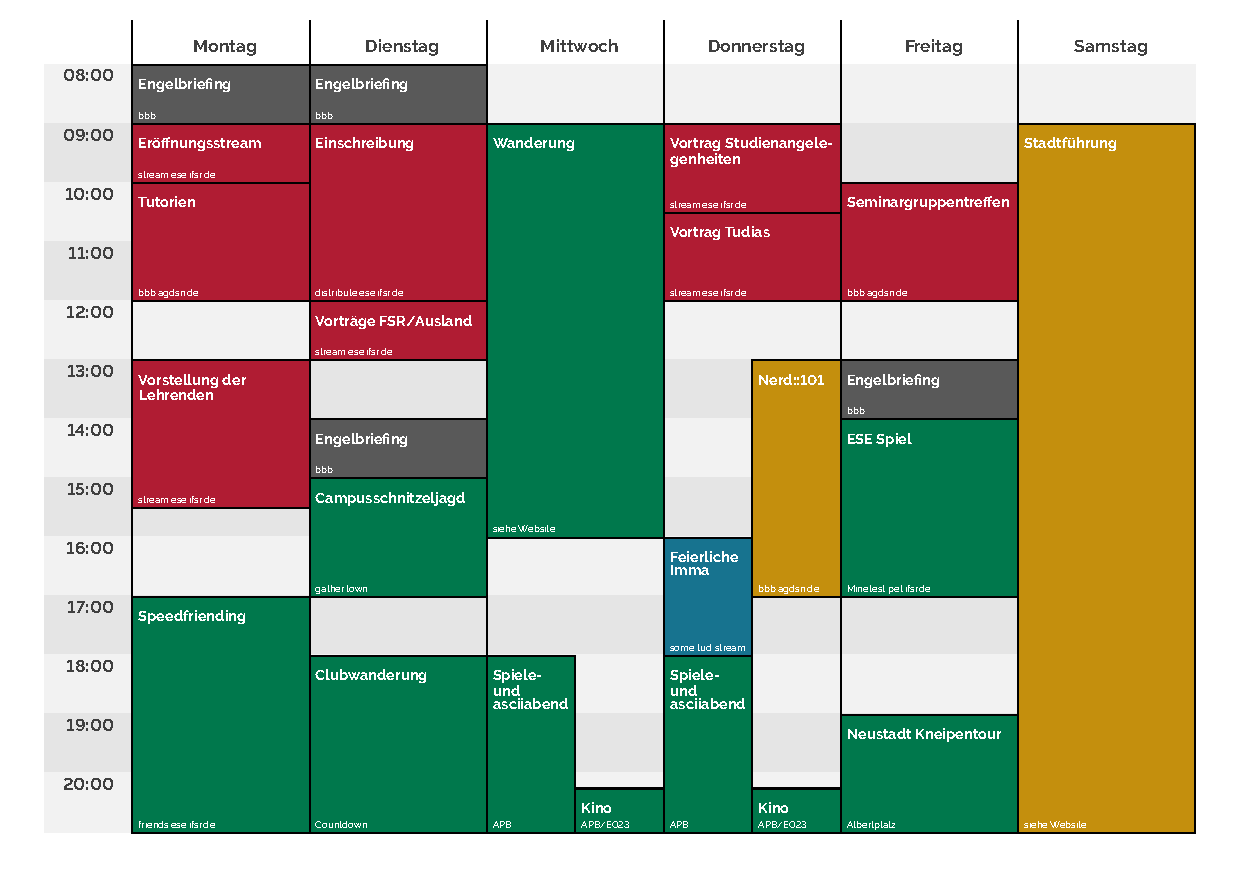
\includepdf[landscape=true]{zeitplan_2020.pdf}


\end{document}
